\documentclass[12pt]{article}
\usepackage[utf8]{inputenc}
\usepackage{array}
\usepackage{xcolor}
\usepackage{graphicx}
\usepackage{mathtools}
\usepackage{amsmath}
\usepackage{multicol}
\usepackage{eqnarray}
\usepackage{wrapfig}


\usepackage{natbib}
\usepackage{hyperref}
\hypersetup{
	colorlinks=true,
	linkcolor=black,
	filecolor=mangeta,      
	urlcolor=blue,
	pdftitle={Overleaf Example},
	pdfpagemode=FullScreen,
}

\usepackage[margin=0.6in]{geometry}

\title{52nd—24th INTERNATIONAL-RUDOLF ORTVAY \\ PROBLEM SOLVING CONTEST IN PHYSICS \\ Problem 10}
\author{Nguyen Thanh Long}
\date{\today}

\begin{document}
	
\maketitle
	
\noindent The potential that given in this problem doesn't have any explicit dependence on coordinates so the momentum of our triatomic molecule is a constant. Therefore, the center of mass frame is a inertial frame of reference, then we will choose this frame with the center of mass is the origin. We can see that the stable equilibrium is a equilateral triangle with egde $L$, so that we will choose the coordinate system as shown below (figure \ref{fig1}) .

\begin{figure}[!htb]
	\centering
	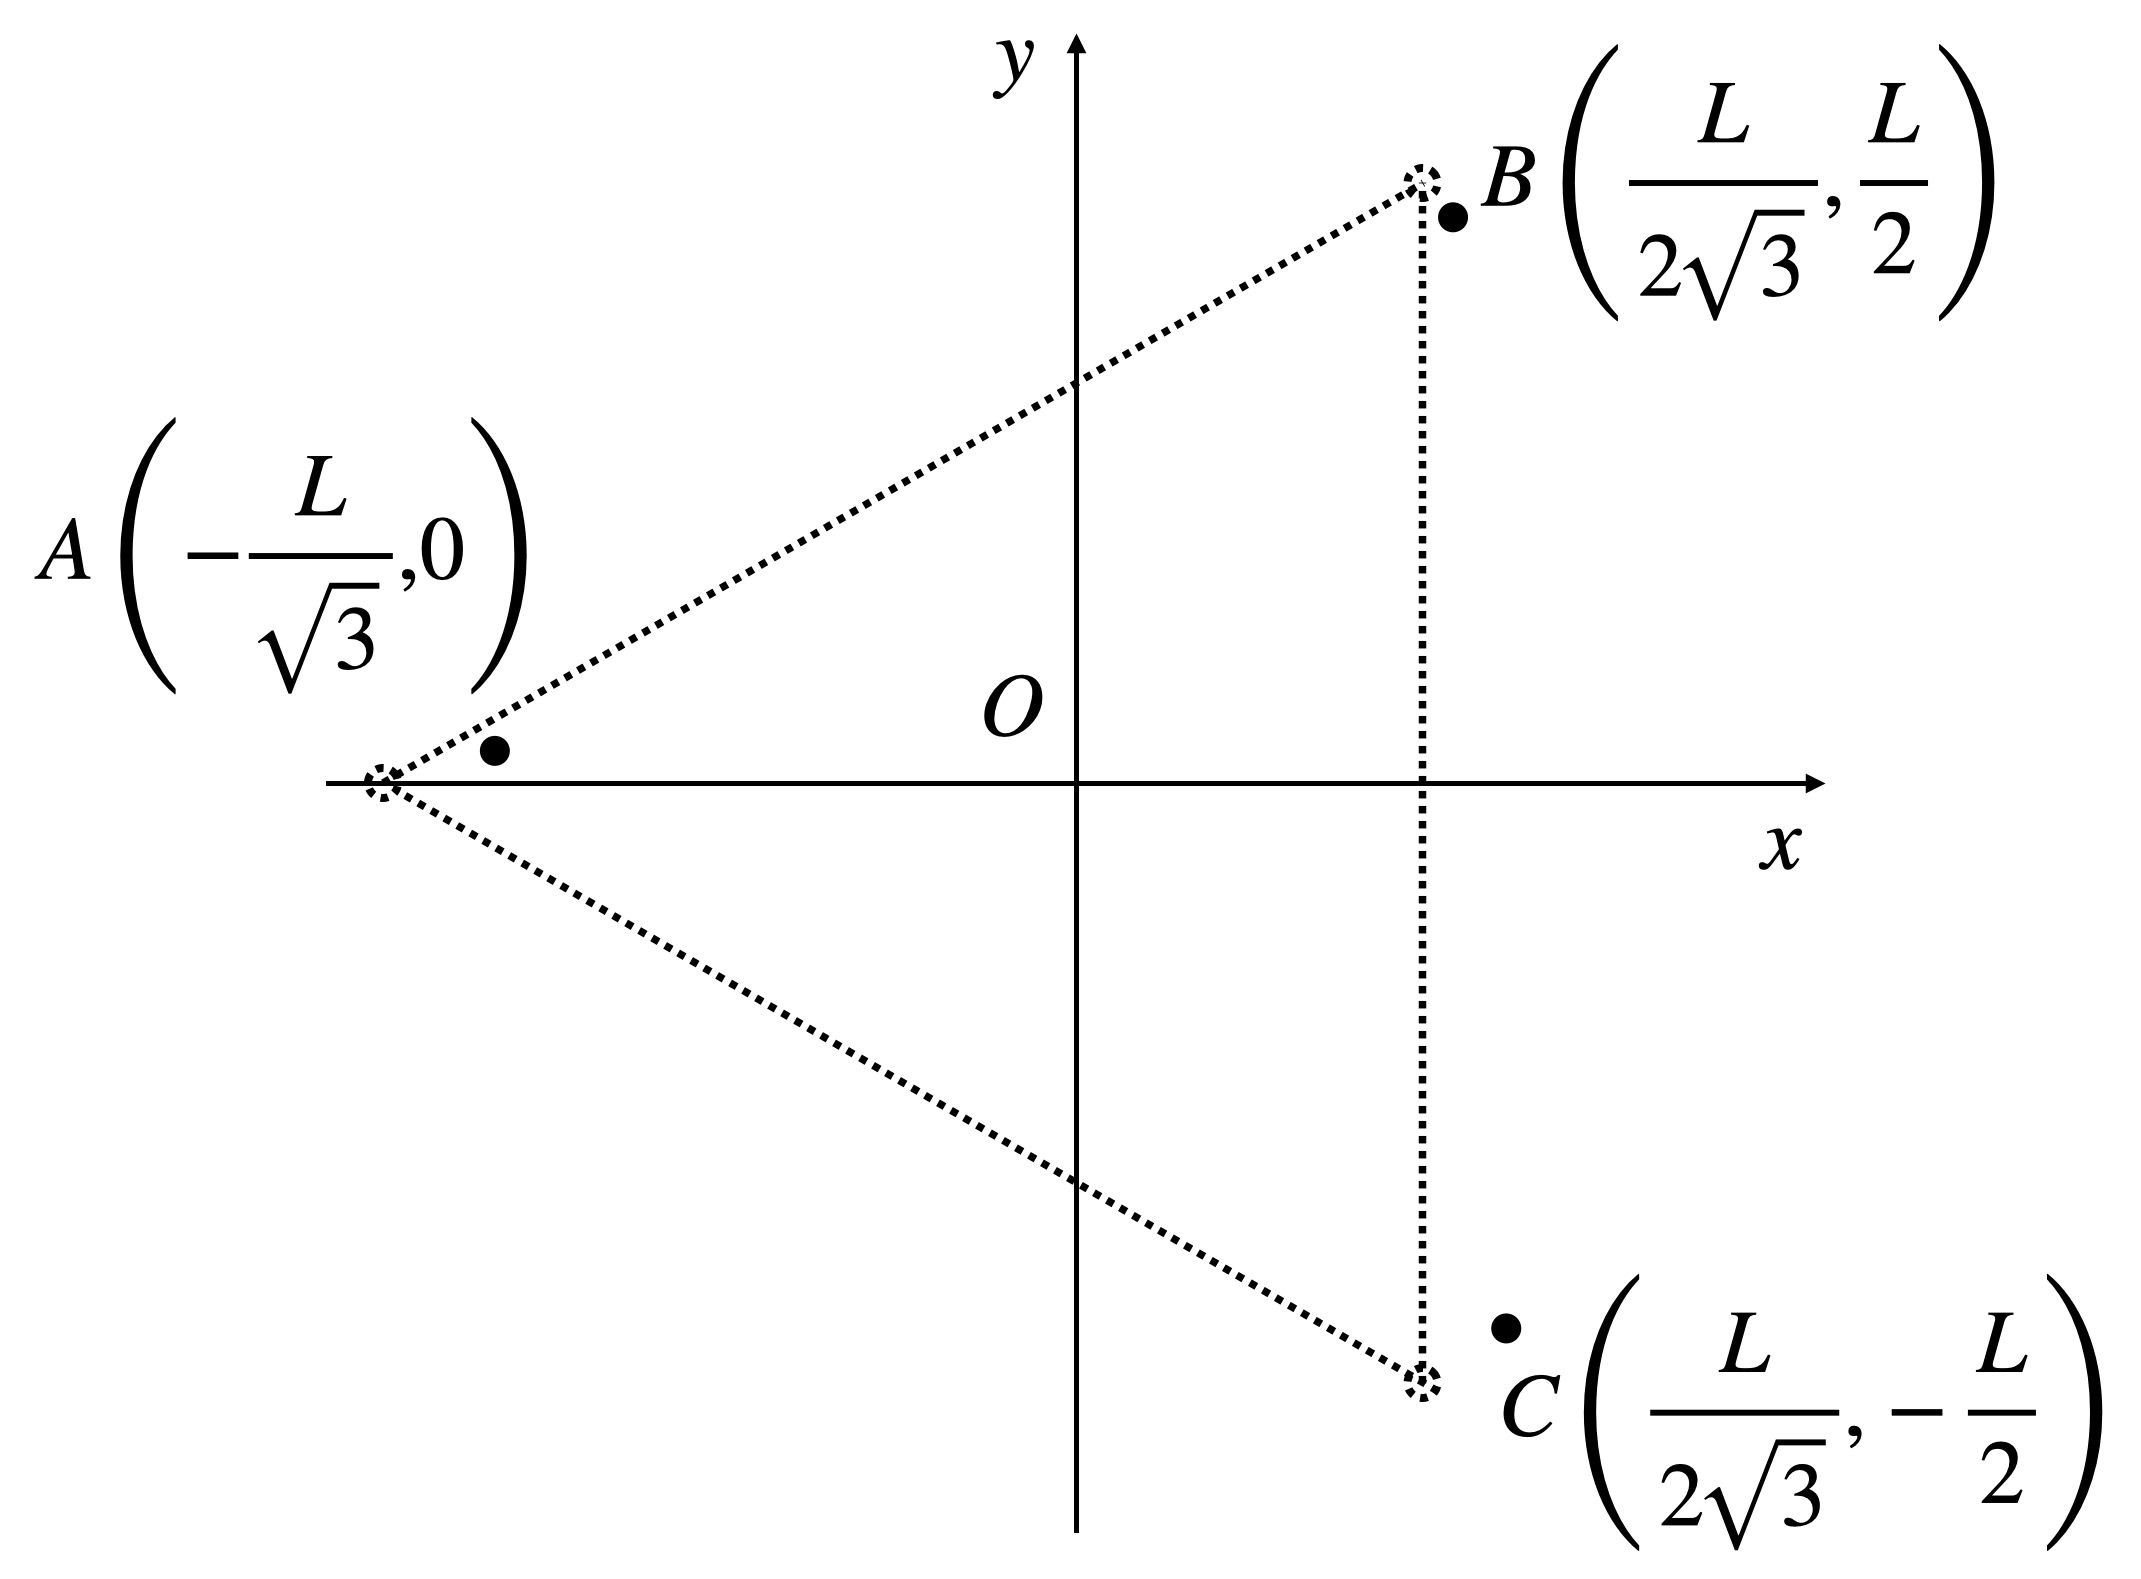
\includegraphics[width=0.7\textwidth]{Fig P10.png}
	\caption{$A$, $B$ and $C$ are three particle of the molecule and dotted line is the equilibrium.}
	\label{fig1}
\end{figure}

\noindent When three particles are moving, the coordinates of them can be write:
\begin{align*}
	& x_B = \frac{L}{2\sqrt{3}}+ \eta_1 .
	& y_B = \frac{L}{2} + \zeta_1 . \\	
	& x_C = \frac{L}{2\sqrt{3}} + \eta_2 .
	& y_C = - \frac{L}{2} + \zeta_2 .\\
	& x_A = - \frac{L}{\sqrt{3}} - \left( \eta_1 + \eta_2 \right) .
	& y_A = - \left( \zeta_1 + \zeta_2 \right) .
\end{align*}	

\noindent Thus, we note the perimeter and area of : 

\begin{align*}
	P & = \sqrt{ \left( x_B - x_A \right)^2 + \left( y_B - y_A \right)^2 } + \sqrt{ \left( x_C - x_A \right)^2 + \left( y_C - y_A \right)^2 } + \sqrt{ \left( x_B - x_C \right)^2 + \left( y_B - y_C \right)^2 } . \\
	A & = \frac{1}{2} \left[ \left( x_C - x_A \right) \left( y_B - y_A \right) - \left( x_B - x_A \right) \left( y_C - y_A \right) \right].	
\end{align*}	

\noindent The Kinetic energy of triatomic molecule:
\begin{align*}
	T & = \frac{1}{2} m \left( \dot{\eta}_1^2 + \dot{\zeta}_1^2 \right) + \frac{1}{2} m \left( \dot{\eta}_2^2 + \dot{\zeta}_2^2 \right) + \frac{1}{2} m \left[ \left( \dot{\eta}_1 + \dot{\eta}_2 \right)^2 + \left( \dot{\zeta}_1 + \dot{\zeta}_2 \right)^2 \right] \\
	& = m \left( \dot{\eta}_1^2 + \dot{\eta}_2^2 + \dot{\eta}_1 \dot{\eta}_2 + \dot{\zeta}_1^2 + \dot{\zeta}_2^2 + \dot{\zeta}_1 \dot{\zeta}_2 \right) .
\end{align*}
\noindent Then the Lagrangian of them is:
$$ L = m \left( \dot{\eta}_1^2 + \dot{\eta}_2^2 + \dot{\eta}_1 \dot{\eta}_2 + \dot{\zeta}_1^2 + \dot{\zeta}_2^2 + \dot{\zeta}_1 \dot{\zeta}_2 \right) - V_0 \left( \frac{P}{L} + \frac{3 \sqrt{3} }{8} \frac{L^2}{A} \right) .$$
\noindent Using the Euler-Lagrange equation $ \frac{d}{dt} \left( \frac{\partial L}{\partial \dot{x} } \right) = \frac{ \partial L}{\partial x} $, we have 4 differential equation: 

\begin{align*}
	2 \ddot{\eta}_1 + \ddot{\eta}_2 & \approx - \frac{V_0}{mL^2} \left( \frac{45}{4} \eta_1 + 9 \eta_2 + \frac{9\sqrt{3}}{4} \zeta_1 \right) . \\
	\ddot{\eta}_1 + 2 \ddot{\eta}_2 & \approx - \frac{V_0}{mL^2} \left( 9 \eta_1 + \frac{45}{4} \eta_2 - \frac{9\sqrt{3}}{4} \zeta_2 \right) . \\
	2 \ddot{\zeta}_1 + \ddot{\zeta}_2 & \approx - \frac{V_0}{mL^2} \left( \frac{9\sqrt{3}}{4} \eta_1 + \frac{27}{4} \zeta_1 \right) . \\
	\ddot{\zeta}_1 + 2 \ddot{\zeta}_2 & \approx - \frac{V_0}{mL^2} \left( - \frac{9\sqrt{3}}{4} \eta_2 + \frac{27}{4} \zeta_2 \right) .
\end{align*}	

\noindent Using matrices, we write them again:

\begin{align*}
	\begin{pmatrix}
		2 & 1 & 0 & 0 \\
		1 & 2 & 0 & 0 \\
		0 & 0 & 2 & 1 \\
		0 & 0 & 1 & 2 
	\end{pmatrix}
	\begin{pmatrix}
		\ddot{\eta}_1 \\
		\ddot{\eta}_2 \\
		\ddot{\zeta}_1 \\
		\ddot{\zeta}_2
	\end{pmatrix}
    = - \frac{V_0}{m L^2}
    \begin{pmatrix}
    	\frac{45}{4} & 9 & \frac{9\sqrt{3}}{4} & 0 \\
    	9 & \frac{45}{4} & 0 & - \frac{9\sqrt{3}}{4} \\
    	\frac{9\sqrt{3}}{4} & 0 & \frac{27}{4} & 0 \\
    	0 & - \frac{9\sqrt{3}}{4} & 0 & \frac{27}{4}
    \end{pmatrix}	
    \begin{pmatrix}
    	\eta_1 \\
    	\eta_2 \\
    	\zeta_1 \\
    	\zeta_2
    \end{pmatrix}
\\ \Rightarrow
   \begin{pmatrix}
   	\ddot{\eta}_1 \\
   	\ddot{\eta}_2 \\
   	\ddot{\zeta}_1 \\
   	\ddot{\zeta}_2
   \end{pmatrix}
    = - \frac{V_0}{m L^2}
    \begin{pmatrix}
    	\frac{9}{2} & \frac{9}{4} & \frac{3\sqrt{3}}{2} & \frac{3\sqrt{3}}{4} \\
    	\frac{9}{4} & \frac{9}{2} & -\frac{3\sqrt{3}}{4} & -\frac{3\sqrt{3}}{2} \\
    	\frac{3\sqrt{3}}{2} & \frac{3\sqrt{3}}{4} & \frac{9}{2} & -\frac{9}{4} \\
    	-\frac{3\sqrt{3}}{4} & - \frac{3\sqrt{3}}{2} & -\frac{9}{4} & \frac{9}{2}
    \end{pmatrix}
    \begin{pmatrix}
    	\eta_1 \\
    	\eta_2 \\
    	\zeta_1 \\
    	\zeta_2
    \end{pmatrix}
\end{align*}

\noindent The vibrational frequencies angular of this molecule $\omega$ satisfy $\ddot{x} = - \omega^2 x$. Thus, $\frac{m \omega^2 L^2}{V_0}$ is the eigenvalues of the matrice:
$$\begin{pmatrix}
	\frac{9}{2} & \frac{9}{4} & \frac{3\sqrt{3}}{2} & \frac{3\sqrt{3}}{4} \\
	\frac{9}{4} & \frac{9}{2} & -\frac{3\sqrt{3}}{4} & -\frac{3\sqrt{3}}{2} \\
	\frac{3\sqrt{3}}{2} & \frac{3\sqrt{3}}{4} & \frac{9}{2} & -\frac{9}{4} \\
	-\frac{3\sqrt{3}}{4} & - \frac{3\sqrt{3}}{2} & -\frac{9}{4} & \frac{9}{2}
\end{pmatrix}$$

\noindent We have found 3 eigenvalues of that matrice: $0$ , $\frac{9}{2}$ (twice), $9$ so that we have 2 frequencies angular of this molecule: $\omega_1 = 3 \sqrt{ \frac{V_0}{m L^2} }$, $\omega_2 = \frac{3}{\sqrt{2}} \sqrt{ \frac{V_0}{m L^2}}$ ( $\omega_3 = 0$ is meaningless so we won't talk about it) Or the vibrational frequencies of this molecule: $f_1 = \frac{3}{2\pi} \sqrt{ \frac{V_0}{m L^2}}$ and $f_2 = \frac{3}{2 \sqrt{2} \pi} \sqrt{ \frac{V_0}{m L^2}}$. \\

\end{document}